\chapter{GPU Programming}
\label{cha:gpu_programming}

In the previous chapter the numerical algorithm and its serial implementation was presented. It discussed various implementation details which have to be considered to arrive at the most efficient implementation.

To further increase the efficiency modern GPUs offer a massively parallel architecture to accelerate many different applications. We will begin with a short introduction to general purpose computing on GPUs. Afterwards, different Application Programming Interfaces (API) for programming on GPUs are discussed regarding their advantages and disadvantages. The chosen API, CUDA, will be presented with its programming model at the end of this chapter.

\section{General Purpose Computing on GPUs}
In the beginning Graphics Processing Units were highly specialized pieces of hardware developed to exclusively improve the performance of real-time 3D graphics. However, in recent years GPUs have started to be used for running arbitrary code instead of being limited to graphics related computations. This allows for impressive performance increases across a wide range of different general purpose applications. A good overview of the evolution of GPU computing can be found in Owens et al.~\cite{Owens2008}.

The deciding factor for the performance is how well the application can be parallelized to take advantage of the massively parallel architecture of GPUs. This massive parallelism has lead to potentially large performance advantages of GPUs over CPUs as illustrated in Fig.~\ref{fig:gpu_performance}. It shows the year over year increase in the theoretical floating point operations per second (FLOP/s). The FLOP/s number is calculated by combining information of the number of compute units, frequency and memory bandwidth for both the CPU and GPU models. This does not necessarily translate to direct real world performance increases but tries to visualize the potential GPUs have.

\begin{figure}[!htbp]
  \centering
  \begin{tikzpicture}
    \begin{axis}[
      title=Theoretical GFLOP/s,
      xlabel={Year},
      ylabel={GFLOP/s},
      date coordinates in=x,
      xticklabel={\year},
      date ZERO=2002-01-01,
      xtick={2002-01-01,2004-01-01,2006-01-01,2008-01-01,2010-01-01,2012-01-01,2014-01-01},
      xmin=2002-01-01,
      xmax=2014-01-01,
      ymin=0,ymax=5500,
      ]
      \addplot[color=set12_light,mark=*,mark options={fill=white}, very thick] table[x=Date,y=Double,col sep=comma,meta=Name] {charts/cpu_performance.csv};
      \addlegendentry{Intel CPU Double Precision}

      \addplot[
      scatter,
      visualization depends on=\thisrow{alignment} \as \alignment,
      nodes near coords,
      point meta=explicit symbolic,
      every node near coord/.style={anchor=\alignment},
      color=set13_light,
      mark=*,
      mark options={fill=white},
      very thick,
      every node near coord/.append style={font=\tiny},
      ] table[x=Date,y=Double,col sep=comma,meta=Name] {charts/double_gpu_performance.csv};
      \addlegendentry{NVIDIA GPU Double Precision}

      \addplot[
      scatter,
      visualization depends on=\thisrow{alignment} \as \alignment,
      nodes near coords,
      point meta=explicit symbolic,
      every node near coord/.style={anchor=\alignment},
      color=set12,
      mark=*,
      mark options={fill=white},
      very thick,
      every node near coord/.append style={font=\tiny},
      ] table[x=Date,y=Single,col sep=comma,meta=Name] {charts/cpu_performance.csv};
      \addlegendentry{Intel CPU Single Precision}
      \addplot[
      scatter,
      visualization depends on=\thisrow{alignment} \as \alignment,
      nodes near coords,
      point meta=explicit symbolic,
      every node near coord/.style={anchor=\alignment},
      color=set13,
      mark=*,
      mark options={fill=white},
      very thick,
      every node near coord/.append style={font=\tiny},
      ] table[x=Date,y=Single,col sep=comma,meta=Name] {charts/single_gpu_performance.csv};
      \addlegendentry{NVIDIA GPU Single Precision}

    \end{axis}
  \end{tikzpicture}
  \caption[Year over year increase in theoretical floating-point operations per second for CPUs and GPUs.]{Year over year increase in theoretical floating-point operations per second for CPUs and GPUs~\cite{CudaProgrammingGuide}.}
  \label{fig:gpu_performance}
\end{figure}

The huge difference in performance between a GPU and a CPU mainly derives from the number of independent compute units. How a compute unit is exactly defined differs between architectures and vendors. On a CPU the number of compute units usually refers to the number of CPU cores. Each individual CPU cores is very fast, however, CPUs usually only have four, eight or maybe sixteen cores. In contrast to this, GPUs can have several hundreds of independent compute units. Each GPU compute unit can perform calculations in parallel and thus provides the opportunity to yield big performance improvements for high-throughput type computations. This is one reason why g general purpose computing on GPUs was introduced to the world of supercomputers. Over time, a growing number of supercomputers started supplementing their computing power with GPUs and some even rely exclusively on GPUs for their computations.

In order to take advantage of these new massively parallel architectures new API had to be developed. The two proposed APIs are OpenCL and CUDA. OpenCL is an open and cross platform standard maintained by the Khronos Group~\cite{OpenCL}. The same group is also responsible for its graphics focused counterpart OpenGL. OpenCL is not exclusive to GPUs, but instead tries to be a general abstract layer for different parallel architectures. This allows OpenCL code to be run not only on GPUs but also on CPUs. CUDA on the other hand is developed by NVIDIA exclusively for their line of GPUs.

\section{CUDA vs. OpenCL}

Choosing between OpenCL and CUDA is the first decision to be made when starting to implement a new project on GPUs. The main advantage of OpenCL is the ability to run on many different devices. All major players in the computing space provide an implementation on top of their platforms. Both Intel and AMD provide the API for their CPU and both AMD and NVIDIA have drivers available for their GPUs. However, this advantage can also be a disadvantage as the achievable performance might suffer from the abstraction across all platforms. The OpenCL framework is potentially not optimized for a particular device specific architecture. CUDA on the contrary is in theory highly optimized to achieve the best possible performance on NVIDIA's GPUs. In practice the difference can possibly be mitigated by spending the extra time to fine-tune the OpenCL implementation to the hardware's specific needs. Another disadvantage of OpenCL is the potentially outdated and inconsistent driver support for the various devices. This is especially true for NVIDIA who seem to have stopped updating OpenCL, still only supporting OpenCL 1.1 which was released back in 2010. Their main focus is on pushing CUDA and updating it to support all the feature in their new GPUs.

For this thesis we chose to go with NVIDIA's CUDA framework mainly because of the available hardware both at the workstation computers and at the local computing cluster. Additionally, this project does not need the cross-platform capability as the main focus is on pure performance in a highly specialized setup and simulation scenario. The application will not be widely distributed and only used for internal purposes.

\section{CUDA Programming Model}
\label{sec:CUDA}
The abbreviation CUDA stands for Compute Unified Device Architecture and was introduced by NVIDIA in 2006 as a general purpose parallel computing platform. It leverages the highly parallel architecture of modern NVIDIA GPUs to solve many different computational problems, which can lead to potentially large performance improvements compared to traditional CPUs.

The CUDA platform allows developers to use a variety of different options to program the GPU. The easiest way is to link to any CUDA-accelerated library and simply using the libraries interfaces from any software environment. For more advanced uses extensions to various programming languages exist like C/C++, Fortran and even managed languages like Java, Python and many more. This allows for easy and fast integration into any software environment the developer is comfortable with. Fig.~\ref{fig:cuda_overview} illustrated the different components of the overall CUDA platform.

\begin{figure}[!htbp]
  \centering
  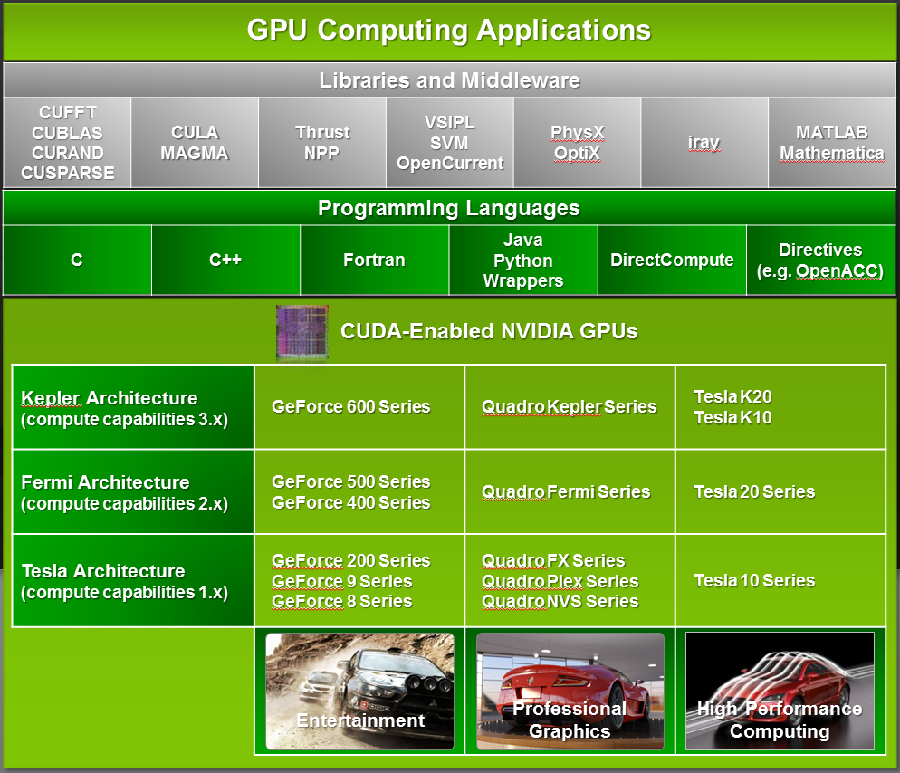
\includegraphics[width=.9\textwidth]{img/cuda_overview.pdf}
  \caption[Overview of the CUDA platform.]{Overview of the CUDA platform~\cite{CudaProgrammingGuide}.}
  \label{fig:cuda_overview}
\end{figure}

The basic building blocks of the CUDA Programming Model from a development perspective are kernels. CUDA kernels are the equivalent of normal C functions. However, the major difference is that instead of being executed just once, kernels are executed in parallel by $N$ different threads. These CUDA threads are distributed and run across the available compute units of the GPU. To illustrate how a very basic kernel invocation looks, Listing~\ref{lst:code_vector_addition} shows a code sample for a very simple vector addition.

\begin{listing}[!htbp]
  \centering
  \inputminted[mathescape,
    linenos,
    numbersep=5pt,
    fontsize=\footnotesize,
    frame=lines,
    framesep=2mm]{c}{lst/cuda_vector_add.lst}
  \caption{Pseudocode for CUDA vector addition.}
  \label{lst:code_vector_addition}
\end{listing}

\paragraph{CUDA Kernels}

It is important to remember that each kernel invocation is executed independently and no ordering is guaranteed. It is therefore essential to avoid any order-dependent operations or shared memory access. There are however, ways to allow for shared memory access which will be briefly touched upon later in the practical implementation of the simulation.

\paragraph{Thread Hierarchy}

In order to efficiently distribute the different threads across the compute units of the GPU, CUDA defines a thread hierarchy. As discussed previously a GPU consists of many independent compute units. On NVIDIA GPUs these units are referred to as Streaming Multiprocessors (SMs). During execution of the application each SM is tasked with running a distinct set of threads. In CUDA these sets of threads are called thread blocks. Each thread block is distributed to all the available SMs, which allows for automatic scalability depending on the number of SMs available  as illustrated in Fig.~\ref{fig:automatic_scaling}. Thus the developer only has to divide the workload into appropriately sized blocks of threads and invoke the kernel.

\begin{figure}[!htbp]
  \centering
  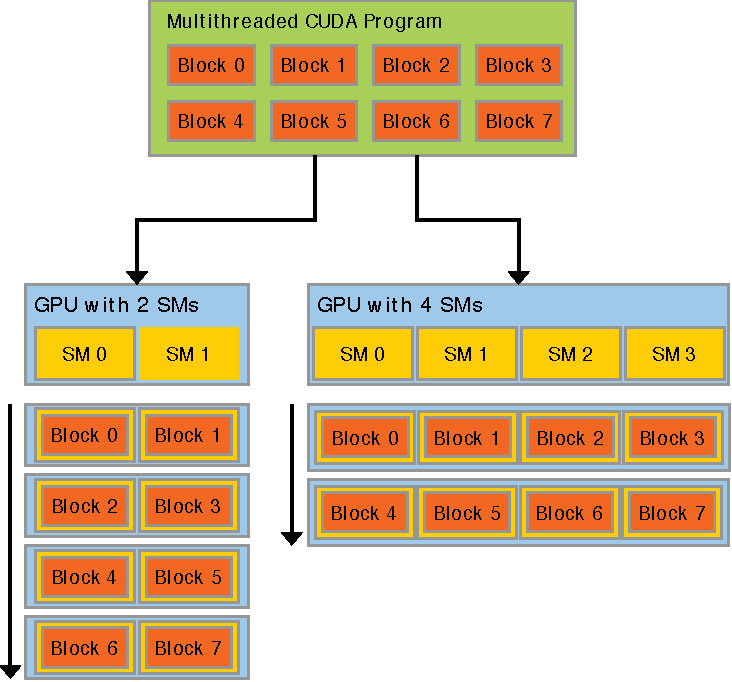
\includegraphics[width=\textwidth]{img/automatic_scaling.pdf}
  \caption[Automatic scaling of blocks across an arbitrary number of Streaming Multiprocessors.]{Automatic scaling of blocks across an arbitrary number of Streaming Multiprocessors~\cite{CudaProgrammingGuide}.}
  \label{fig:automatic_scaling}
\end{figure}

How to choose the optimal size of a block in order to maximize the performance is not an easy question to answer and it is highly dependent on the particular task and implementation. In practice the size is often chosen by running benchmarks with various sizes to determine the optimal configuration.

In order to make programming easier, CUDA blocks can be addressed using either a one-dimensional, two-dimensional, or three-dimensional thread index. For example in the case of a calculation involving matrices, it is more natural to think about parallelizing each element given by the row and column index instead of a single one-dimensional index. This is illustrated in the code sample in Listing~\ref{lst:code_matrix_addition}

\begin{listing}[!htbp]
  \centering
  \inputminted[mathescape,
    linenos,
    numbersep=5pt,
    fontsize=\footnotesize,
    frame=lines,
    framesep=2mm]{c}{lst/cuda_matrix_add.lst}
  \caption{Pseudocode for CUDA matrix addition, illustrating 2D thread blocks.}
  \label{lst:code_matrix_addition}
\end{listing}

Finally, as the resources of each Streaming Multiprocessor are limited, there is an upper bound of how many threads a block can contain. Currently this maximum number of threads is $1024$. This means that the maximum size of matrices, that can be added with the two-dimensional thread block code sample in Listing~\ref{lst:code_matrix_addition} is $32\times32 = 1024$. To solve this problem CUDA introduces another layer above blocks called a grid. A grid organizes thread blocks again into either one, two, or three dimensions. The number of thread blocks in a grid is unlimited and thus solely dependent on the size of the workload. Fig.~\ref{fig:grid_blocks} shows an example configuration of a 2D grid with 2D blocks.

\begin{figure}[!htbp]
  \centering
  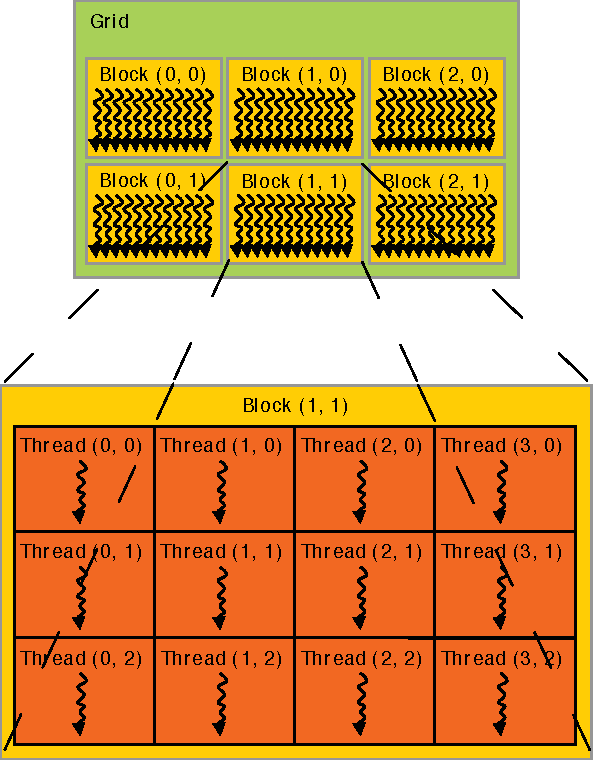
\includegraphics[width=0.6\textwidth]{img/grid_blocks.pdf}
  \caption[CUDA block addressing using 2D grid with 2D thread blocks.]{CUDA block addressing using 2D grid with 2D thread blocks~\cite{CudaProgrammingGuide}.}
  \label{fig:grid_blocks}
\end{figure}

\paragraph{Memory Hierarchy}

In addition to the \emph{Thread Hierarchy} CUDA also implements a 3 layer memory hierarchy as illustrated in Fig.~\ref{fig:memory_hierarchy}. Each level of this hierarchy differs in size, latency and scope. The sizes refers to amount of bytes that can be stored in the level and latency to the time it between requesting data and being able to actually use it. Additionally each level is confined to a specific scope, restricting from where the data can be accessed.

The first level contains the fastest and smallest memory. This is a private memory where each thread has its own area and only this thread can read from and write to this area. How much space each thread has is determined by how many threads are executed on each SM. The more memory an individual thread requires the fewer threads can run in parallel on a SM. Optimizing this trade-off is important for achieving a good performance. On the newest GPUs each SM has $65536 * 32\text{-bit} = 256\text{KB}$ to divide among the threads.

The second level is called shared memory, or sometimes local memory. Although it is slower than the private memory, it has the advantage that all threads executing on an SM have simultaneous access to it. This allows different threads to cooperate and share work. Depending on the characteristics of the algorithm, this can save a lot of computing time. Therefore it is important to analyze whether shared memory can actually improve the performance. The size of this memory level on current GPUs is around $64\text{KB}$ to $96\text{KB}$.

The third level contains the largest memory area which is called the global memory. This is the amount of memory used  on the packaging of the GPUs to advertise the product. Nowadays it is usually $2\text{GB}$ or $4\text{GB}$. It is accessible by all threads and stores all data relating to the current application. However, accessing it can be quite slow compared to the other levels of the memory hierarchy. Additionally, one has to be careful to avoid memory conflicts when accessing the same memory location form different threads at the same time. This is especially important since this can further reduce the performance. Taking everything into account, it can be said that it is an important optimization step to make access to global memory as efficient as possible. This can be achieved by intelligently packing data, or caching data in a lower level of the hierarchy. 

Another option to avoid the slow the performance of the global memory is to make sure that the required data for each individual thread from global memory is small enough. The associated latency when reading data from global memory can be hidden when enough calculation are performed on this data. The GPU is then able to quickly switch to another set of threads and continue the computation while waiting on data from global memory.

\begin{figure}[!htbp]
  \centering
  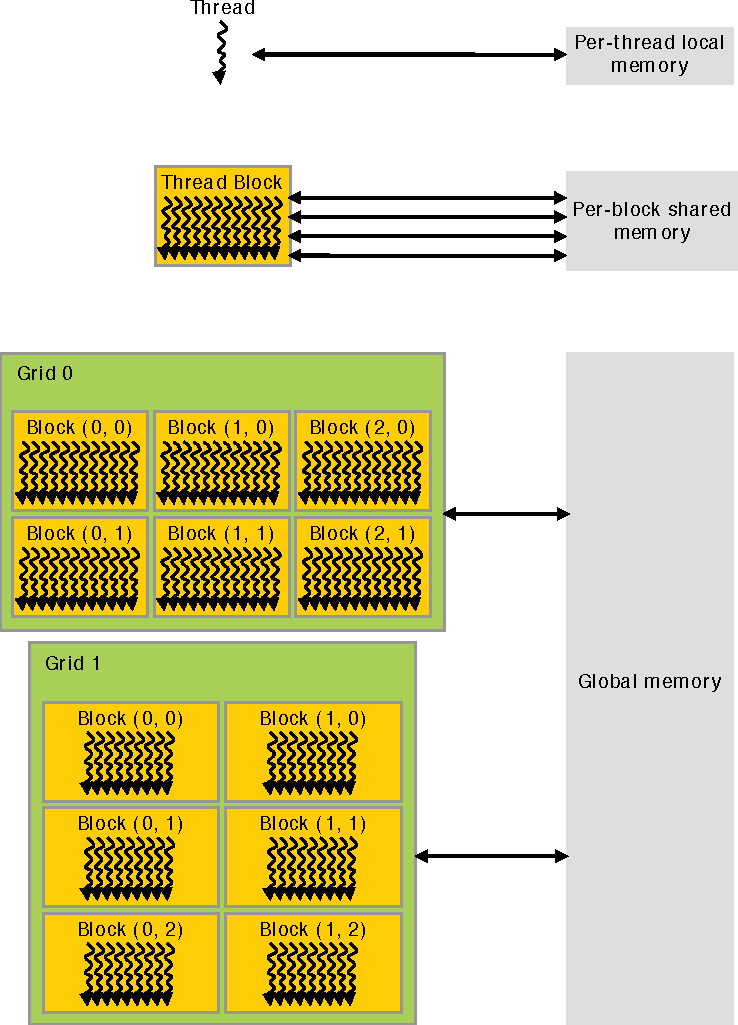
\includegraphics[width=0.8\textwidth]{img/memory_hierarchy.pdf}
  \caption[CUDA memory hierarchy.]{CUDA memory hierarchy~\cite{CudaProgrammingGuide}.}
  \label{fig:memory_hierarchy}
\end{figure}
